% ============================================================================
%  Federated and meta-learned blood-glucose forecasting across sites
%  PLOS Digital Health submission (PLOS template v3.8 Apr 2026)
%
%  STATUS: Full coherent draft. Abstract, Author summary, Introduction,
%  Materials and methods, Results (incl. finetuning), and Discussion (incl.
%  external-comparison subsection) written. Under reviewer-style revision.
%
%  NOTE: this uses the PLOS class options and the `cite` package (numeric
%  Vancouver citations). The bibliography style is `plos2015` (the genuine PLOS
%  Vancouver BibTeX style; the current template ships an identical file renamed
%  plos2025.bst). plos2015.bst is committed alongside this .tex so it compiles
%  as-is on Overleaf. The bib database is references.bib.
% ============================================================================
\documentclass[10pt,letterpaper]{article}
\usepackage[top=0.85in,left=2.75in,footskip=0.75in]{geometry}

\usepackage{amsmath,amssymb}
\usepackage{changepage}
\usepackage{textcomp,marvosym}
\usepackage{cite}
\usepackage{nameref,hyperref}
\usepackage[right]{lineno}
\usepackage[nopatch=eqnum]{microtype}
\DisableLigatures[f]{encoding = *, family = * }
\usepackage[table]{xcolor}
\usepackage{array}

\newcolumntype{+}{!{\vrule width 2pt}}
\newlength\savedwidth
\newcommand\thickcline[1]{%
  \noalign{\global\savedwidth\arrayrulewidth\global\arrayrulewidth 2pt}%
  \cline{#1}%
  \noalign{\vskip\arrayrulewidth}%
  \noalign{\global\arrayrulewidth\savedwidth}%
}
\newcommand\thickhline{\noalign{\global\savedwidth\arrayrulewidth\global\arrayrulewidth 2pt}%
\hline
\noalign{\global\arrayrulewidth\savedwidth}}

% Text layout
\raggedright
\setlength{\parindent}{0.5cm}
\textwidth 5.25in
\textheight 8.75in

\usepackage[aboveskip=1pt,labelfont=bf,labelsep=period,justification=raggedright,singlelinecheck=off]{caption}
\renewcommand{\figurename}{Fig}

\bibliographystyle{plos2015}

\makeatletter
\renewcommand{\@biblabel}[1]{\quad#1.}
\makeatother

% Header and Footer with logo
\usepackage{lastpage,fancyhdr,graphicx}
\usepackage{epstopdf}
\pagestyle{fancy}
\fancyhf{}
\rfoot{\thepage/\pageref{LastPage}}
\renewcommand{\headrulewidth}{0pt}
\renewcommand{\footrule}{\hrule height 2pt \vspace{2mm}}
\fancyheadoffset[L]{2.25in}
\fancyfootoffset[L]{2.25in}
\lfoot{\today}

\begin{document}
\vspace*{0.2in}

% Title must be 250 characters or less. Sentence case.
\begin{flushleft}
{\Large
\textbf{Federated and meta-learned blood-glucose forecasting across sites: a domain-generalisation benchmark and a four-institution deployment}
}
\newline
\\
Name1 Surname\textsuperscript{1*}
\\
\bigskip
\textbf{1} Affiliation Dept/Program/Center, Institution Name, City, State, Country
\\
\bigskip

* correspondingauthor@institute.edu

\end{flushleft}

% Please keep the abstract below 300 words
\section*{Abstract}
Algorithms that forecast blood glucose 30 minutes ahead are used in type~1
diabetes (T1D) to warn of excursions, but a model trained at one centre can
transfer poorly to new patients and sites --- and the varied data that would
make it robust cannot lawfully be pooled. Federated learning (FL)
trains a shared model without moving raw records. For glucose forecasting, FL
strategies have rarely been compared head-to-head, evaluations
seldom separate accuracy on the training cohorts (held-in) from accuracy on
unseen cohorts (out-of-distribution, OOD), and almost all such work is
simulated. Using one encoder--decoder transformer, four real T1D cohorts as
federated clients and three never-seen cohorts (ReplaceBG, BrisT1D, Flair) as
OOD tests, we benchmarked single-cohort local training against federated
averaging (FedAvg), FedProx, meta-learning for domain generalisation (MLDG),
and two personalised-FL methods under a by-patient split over five seeds,
reporting held-in and OOD error at 30 and 60 minutes.

The privacy constraint proved nearly free. Federation reached $19.99$ mg/dL
RMSE at 30 minutes against $19.90$ for a convergence-matched model trained on
the four cohorts pooled --- a gap of $0.09$ mg/dL, under $1\%$ of the
$12$--$14$ mg/dL error of the CGM sensors these models read.
Out-of-distribution, the best single-cohort model matched the federated
models, but the model trained on the smallest cohort collapsed on all three
($28.5$ vs $\approx$$21.3$ mg/dL on ReplaceBG) with in-domain accuracy that
gave no warning. On ReplaceBG the federated model reached $21.34$ mg/dL
without seeing any of its patients, within the range of models trained on it.
A new site beat from-scratch training on all its patients after finetuning on
$9$--$17$ of them. Differences between FL strategies fell within seed noise.
We ran the federation live across four universities, not in simulation, using
tooling light enough for a small group of clinics to adopt.

% Author Summary: 150-200 words, first person.
\section*{Author summary}
People with type~1 diabetes increasingly rely on algorithms that predict their
glucose half an hour ahead. These work well for the patients they were trained
on but can fail on a different clinic or population, and the data that would
fix that sits in institutions which cannot legally pool raw records. Federated
learning lets them train a shared model while each keeps its data in-house.

We treated four diabetes studies as collaborating sites, compared the main
federated methods, and tested each on three further studies that gave no
training data. Federation cost almost nothing: it came within $0.09$ mg/dL of a
model trained on all four datasets pooled, far less than the error of the
sensors themselves. Training on one cohort alone was a gamble --- the best such
model matched federation, another failed on every unseen population, and their
accuracy at home gave no warning. A new site could beat training alone after
finetuning the shared model on as few as nine of its own patients.

We ran this across four universities for real, each holding only its own data.
That gives a small group of clinics a practical route to predictors that fail
less often on unseen patients.

\clearpage
\newgeometry{top=0.85in,left=1in,right=1in,footskip=0.75in}
\linenumbers

% ===========================================================================
\section*{Introduction}

Type~1 diabetes (T1D) affects an estimated 8.4~million people worldwide and its
incidence is rising in many regions~\cite{idf2021,gregory2022t1dindex}. People living with T1D must
continually balance insulin, food, and activity to keep blood glucose within a
narrow target range; sustained excursions above or below that range drive both
the acute dangers of hypoglycaemia and the long-term microvascular and
cardiovascular complications of hyperglycaemia. Continuous glucose monitoring
(CGM), which reports interstitial glucose roughly every five minutes, is now
central to diabetes care; it underpins clinical outcomes such as time in range,
for which international consensus targets have been defined~\cite{battelino2019tir}. The same dense data stream makes
short-horizon glucose \emph{forecasting} clinically valuable: a reliable
prediction of where glucose will be in 30--60 minutes can trigger preemptive
alerts, inform bolus and snack decisions, and close the loop in automated
insulin-delivery systems~\cite{vettoretti2020advanced,bekiari2018ap}.

Short-horizon CGM forecasting has progressed from autoregressive and classical
machine-learning models to deep sequence models. Recurrent architectures with
predictive variance estimation established strong baselines on benchmark
cohorts~\cite{martinsson2020}, and standardised datasets and challenges shaped
much of the early evaluation~\cite{marling2020ohio}. The
transformer~\cite{vaswani2017attention} and its long-horizon time-series
variants~\cite{zhou2021informer,wu2021autoformer} have since been adapted to
glucose, with personalised, uncertainty-aware transformer forecasters reporting
state-of-the-art accuracy~\cite{sergazinov2023gluformer} and curated CGM
benchmarks standardising their evaluation~\cite{sergazinov2024glucobench}.
These models are accurate when trained and evaluated on the same cohort, but how
well they transfer across cohorts is an open question~\cite{ghimire2024generalize}:
glucose dynamics, demographics, and devices differ from site to site, and a model
can degrade on populations it did not see in training~\cite{farahmand2025glumind}.
A model that has only seen one cohort therefore has little reason to generalise to
the next; robust generalisation instead calls for training over large, diverse
populations spanning many sites.

Large, diverse training data is exactly what is hardest to assemble. CGM traces
are sensitive personal health records, fragmented across hospitals, clinical
trials, device manufacturers, and national registries, and governed by
data-protection regimes such as the GDPR and HIPAA that restrict moving raw
records between institutions, let alone across borders. The data that improve
generalisation and the data that exist are thus mismatched: large, heterogeneous
corpora are what is needed, but what is available is many small, governed silos.
Federated learning (FL) addresses this tension~\cite{mcmahan2017fedavg}: sites
train on their own data and exchange only model updates, so a shared model is
learned without any raw record leaving its institution. On this basis FL has been
widely adopted for collaborative medical machine
learning~\cite{rieke2020future,sheller2020federated,kaissis2020secure}. Its
central difficulty is statistical heterogeneity: plain federated averaging
degrades when client distributions diverge, motivating proximal
regularisation~\cite{li2020fedprox} and control-variate variance
reduction~\cite{karimireddy2020scaffold}. Most of this work, however, is evaluated
in simulation, where ``clients'' are partitions of one dataset on a single
machine.

Even with federation, real CGM cohorts differ in device generation, demographics,
treatment protocols, and glycaemic regime, and these differences widen across
countries. A federated model must therefore cope with substantial domain shift: it
should generalise to patients, and even whole cohorts, it never trained on (domain
generalisation), and/or specialise to each site (personalisation). Domain
generalisation seeks models that transfer to unseen
distributions~\cite{zhou2022dgsurvey}, and meta-learning for domain generalisation
(MLDG) simulates train/test domain shift within each update so the model learns to
generalise rather than memorise~\cite{li2018mldg}.

These ideas have already reached glucose forecasting in the \emph{centralised}
setting: a Transformer trained with MLDG on a single large cohort transfers
zero-shot to external cohorts~\cite{zhu2024gpformer}, and a language-model
backbone with insulin and electronic-health-record inputs improves in-cohort
accuracy further~\cite{zhu2026glullm}. What this line of work does \emph{not}
address is the constraint that motivates this paper: the models are trained
centrally, on data pooled at a single site, which is precisely what
data-protection regimes prevent a multi-institution consortium from doing. Our
question is therefore what happens when the same objective must be
optimised \emph{without pooling} --- across several institutions that each hold a
different cohort and cannot exchange raw records --- and how the federated
alternatives compare with one another under that constraint.

Bringing domain generalisation into federation is an active area surveyed by Li
et al.~\cite{li2025fedDGsurvey}, spanning several families. Meta-learning approaches adapt the model-agnostic
meta-learning objective to federation, for communication-efficient
convergence~\cite{chen2018fedmeta} or for models that personalise to a new client
in a few gradient steps~\cite{fallah2020perfedavg}. Personalisation approaches keep
a per-client model: APFL learns an adaptive convex mixture of the global and a
local model~\cite{deng2020apfl}, while Ditto regularises each client's personal
model toward the global one with a tunable proximal strength~\cite{li2021ditto}.
Other approaches instead align client representations, via model-contrastive
objectives~\cite{li2021moon}, federated contrastive learning for multi-centre
medical imaging~\cite{fedcl2023}, or adversarial domain
alignment~\cite{flda2023,fedadv2022}. Our benchmark covers the first two
families---meta-learning (MLDG) and personalisation (APFL, Ditto)---alongside
standard federated averaging (FedAvg, FedProx) and single-cohort local training,
and leaves representation-alignment methods to future work.

\textbf{Yet these methods are rarely compared head-to-head for glucose
forecasting.} They are seldom benchmarked against one another on a common task, and
evaluations rarely separate the two regimes that matter clinically---accuracy on
patients from the training cohorts (held-in) versus accuracy on entirely unseen
cohorts (out of distribution, OOD)---even though a method can behave quite
differently in the two. Closing this gap---comparing federated strategies on one
glucose task under a shared protocol, with held-in and OOD performance reported
separately---is the main focus of this paper.

A second, more practical observation is that almost all federated glucose work is
simulated rather than deployed, with ``clients'' as partitions of one dataset on a
single machine. Running a federation for real additionally requires networked,
physically separate sites to exchange updates and to start from a common model;
production FL frameworks can do this but carry substantial dependencies and
assumptions that can be ill-suited to a small clinical consortium that simply wants
a handful of sites, one cohort each, to train together. We therefore also ask a
feasibility question: whether a lightweight cross-site federation for CGM
forecasting can be built and run across real machines with minimal tooling.

This paper makes three contributions.

\textbf{First, a controlled domain-generalisation benchmark of federated
strategies for transformer-based glucose forecasting.} Using a common
encoder--decoder transformer and four real adult T1D cohorts as federated
clients, with three held-out cohorts as OOD test sites, we compare single-cohort
local training, FedAvg, FedProx, MLDG, and two personalised-FL methods (APFL and
Ditto) under a multi-seed protocol, reporting held-in and OOD accuracy separately
at the 30- and 60-minute horizons --- 30 minutes being the horizon most commonly
used for preemptive glucose alerts. Two choices make this a stricter test than is
usual in this literature. We split strictly \emph{by patient}, so every reported
error measures generalisation to people the model has never seen, rather than the
by-time split that most prior work on these cohorts uses; and we hold the
architecture fixed across every strategy, so the comparison isolates the training
strategy rather than model capacity. Under that protocol our zero-shot federated
model reaches an error on ReplaceBG that sits inside the field of models developed
\emph{on} ReplaceBG, without having seen any of its patients --- though this parity
holds at 30 minutes and not at 60, where cohort-specific behaviour matters more.
All cohorts are adult T1D populations, so our findings should not be assumed to
extend to paediatric or type-2 diabetes.

\textbf{Second, a recipe for onboarding a new site: federate, then adapt.} The
benchmark identifies a tension --- generalising across sites transfers well but
leaves per-site accuracy on the table, while specialising to a site forfeits that
transfer --- and we show it can be resolved by treating the federated model as a
foundation rather than a finished product. Finetuning the global model on a new
cohort's own patients beats training there from scratch on all three held-out
cohorts, by $0.3$--$0.7$ mg/dL, and needs as little as $10\%$ of that cohort's
patients to do so: seventeen individuals on the largest held-out cohort, two on
the smallest. A centre joining after training can therefore reach, and exceed,
local-only performance without a large local data-collection effort, which is what
turns the benchmark into usable deployment advice.

\textbf{Third, we run this federation for real across four institutions, rather
than simulating it.} We build, from scratch, a lightweight
cross-site FL system for CGM forecasting: a stateless aggregation server that
holds the global model but no data, and clients that each wrap one institution's
cohort, communicating over HTTP using only the Python standard library. The server
broadcasts the initial weights so every client starts from an identical model, and
the same protocol carries FedAvg, FedProx, and MLDG training. The results we
report were produced by running this system live across four UK universities ---
University College London, the University of Manchester, Newcastle University, and
the University of Oxford --- with one client per institution, each training only on
its own cohort and exchanging nothing but model weights over the public internet.
This exercises the conditions a real consortium faces (separate administrative
domains, separate hardware, network round-trips between rounds) rather than the
single-host shortcut that almost all federated glucose work takes. What we do
\emph{not} claim is a production-grade or cross-border deployment: the system
carries no encryption, secure aggregation, or differential privacy, and all four
sites are in one country, so the additional legal machinery of cross-jurisdiction
federation is untested. Those are engineering and governance gaps, not
architectural ones, and we return to them in the Discussion.

Taken together, the benchmark shows how to evaluate federated glucose forecasting
and what such an evaluation reveals, the finetuning results show what a
new site should do with the resulting model, and the deployment shows that a
federation of this kind runs across four real institutions, not only in
simulation.

% ===========================================================================
\section*{Materials and methods}

\subsection*{Datasets and federation setup}

We use seven type-1 diabetes (T1D) continuous glucose
monitoring (CGM) datasets (see Data and code availability for access routes). Four serve as the federated clients --- HUPA-UCM
\cite{hidalgo2024hupaucm}, ABC4D \cite{abc4d_nct}, ARISES \cite{zhu2022arises},
and T1D-UOM \cite{alsuhaymi2025t1duom} --- with \emph{one dataset per client}. Each dataset
originates from a distinct study, population, and device, so a per-dataset
partition makes every client a genuinely different domain rather than an
arbitrary shard of a pooled corpus; this is what lets the federation function as
a test of cross-domain generalisation. The remaining three datasets ---
ReplaceBG \cite{aleppo2017replacebg}, BrisT1D \cite{james2025brist1d}, and Flair
\cite{jaeb_flair} --- are never seen
during training and are used only as held-out, out-of-distribution (OOD) test
cohorts. Within
each client, we partition patients
into disjoint train, validation, and test groups, splitting strictly by
patient ID so that no patient contributes data to more than one group. Reported performance therefore measures generalisation to
unseen patients rather than to unseen windows of patients already observed.

Five of the seven cohorts --- the clients HUPA-UCM and T1D-UOM, and all three
held-out cohorts (ReplaceBG, BrisT1D, and Flair) --- are obtained through
MetaboNet \cite{wolff2026metabonet}, a
recently released resource that consolidates public T1D datasets into a single
harmonised schema on a common 5-minute grid; the remaining two client cohorts,
ABC4D and ARISES, are converted
into the same schema from their original releases. Patient counts in
Table~\ref{tab:datasets} are therefore those of the data release we use, which
for the MetaboNet-derived cohorts are smaller than the totals in the source
publications (HUPA-UCM: 22 of the 25 published; T1D-UOM: 14 of the 17
published). We do not adopt MetaboNet's own train/test split, which allows the
same patient to appear in both partitions; instead we re-split strictly by
patient as described above.

Table~\ref{tab:datasets} summarises each cohort. Mean and standard deviation of
CGM are reported in mg/dL, and time-in-range (TIR) is the fraction of CGM
readings in the clinical 70--180 mg/dL band.

\begin{table}[!ht]
\centering
\captionsetup{justification=centering,singlelinecheck=on}
\caption{\bf Federated client cohorts.}
\label{tab:datasets}
\begin{tabular}{lrrrrr}
\thickhline
dataset & patients & total windows & mean CGM & sd CGM & TIR (\%) \\
        &          &               & (mg/dL)  & (mg/dL) & 70--180  \\
\hline
HUPA-UCM & 22 & 291,728 & 140.9 & 56.6 & 72.2 \\
ABC4D    & 25 & 562,043 & 155.1 & 63.4 & 65.5 \\
ARISES   & 12 & 126,248 & 160.5 & 63.7 & 63.7 \\
T1D-UOM  & 14 & 300,796 & 151.6 & 59.9 & 70.5 \\
\thickhline
\end{tabular}
\begin{center}
{\small The three OOD test cohorts (ReplaceBG, BrisT1D, Flair) are excluded from
training and reported separately (Table~\ref{tab:ood}). ARISES is both the
highest-glucose and the smallest client cohort. Patient counts are those of the
data release we use (see text); for HUPA-UCM and T1D-UOM they are smaller than
the totals in the original dataset publications.}
\end{center}
\end{table}

\subsection*{Preprocessing and windowing}

Every cohort is resampled to a uniform 5-minute grid. We form supervised
examples with a sliding window of 72 samples (6\,h) of CGM context to forecast
the next 12 samples (60\,min), advancing the window one sample at a time
(stride~1). Windows that would bridge a sensor gap longer than 6 samples
(30\,min) are discarded, so every example is contiguous. CGM is normalised with
a single \emph{global} mean and standard deviation ($154.04 \pm 61.00$ mg/dL)
computed from the four training cohorts only and shared
across all clients. A common
normalisation keeps the global model's input scale identical at every site,
which is what allows weights aggregated across clients to be applied directly to
the OOD cohorts. Alongside CGM,
each example carries a time-of-day mark encoded
as $(\sin 2\pi\,\mathrm{frac},\ \cos 2\pi\,\mathrm{frac})$, where $\mathrm{frac}$
is the fraction of the day, to expose circadian structure.

\subsection*{Forecasting model}

The forecaster is a standard Informer-style sequence-to-sequence
(encoder--decoder) Transformer~\cite{zhou2021informer} that maps
the 72-step CGM context to the 12-step horizon, using \emph{full}
(dense) scaled dot-product attention.
Holding this architecture fixed across every client and every federated
strategy is what lets our comparisons isolate the \emph{training} strategy rather
than the model. It uses
$d_{\text{model}}=128$, 8 attention heads, 6 encoder layers, 2 decoder layers,
feed-forward width $d_{\text{ff}}=2048$, ReLU activations, and dropout~$0.05$
($\approx 4.9$\,M parameters). Decoding is single-shot rather than
autoregressive, following the Informer convention~\cite{zhou2021informer}: the
decoder input is a warm-up of the last $\texttt{label\_len}=6$ CGM samples
(30\,min) of the context concatenated with 12 zero placeholders for the horizon,
and the corresponding time-of-day marks are supplied for all 18 decoder
positions --- as in GPFormer~\cite{zhu2024gpformer} --- so the decoder sees the
calendar time of the steps it must predict but
none of their glucose values. The decoder predicts a single CGM channel ($c_{\text{out}}=1$) and the
model is trained with mean-squared-error (MSE) loss. The model emits a point
forecast only; it produces no predictive-uncertainty estimate (see Limitations).

\subsection*{Federated learning system}

Training is coordinated by a from-scratch, networked federated learning system
in which one institution runs a server and each cohort runs a client. The server
holds the global model weights but never sees any data: at round one it mints a
single seeded set of initial weights and broadcasts them, so every client begins
from byte-identical parameters regardless of hardware. Each round, clients fetch
the current global weights, train locally on their own cohort, and return updated
weights; the server aggregates them by FedAvg and advances to the next round.
Clients communicate with the server over plain HTTP through a small task
state-machine (train\,$\rightarrow$\,validate\,$\rightarrow$\,test), so the same
protocol carries FedAvg, FedProx, and MLDG without modification --- the choice of
strategy is entirely client-side, and the server always performs the same FedAvg
aggregation.

The federation is geographically distributed: the four clients are run at four different UK institutions --- University College
London, the University of Manchester, Newcastle University, and the University of
Oxford --- with one client per institution, and the aggregation server hosted at one of the sites. All coordination happens
over the public internet, so the system exercises the real conditions a clinical
consortium would face (separate administrative domains, separate hardware,
network round-trips between rounds) rather than the shared-memory shortcut that
most federated glucose studies take. The system nevertheless uses plain HTTP
without encryption, secure aggregation, or differential privacy; it demonstrates
the training workflow across real institutions, not a production-grade secure
channel (see Limitations).

\subsection*{Federated strategies and baselines}

\textbf{Local (baseline).} Our primary comparator is local training: a separate
model trained on a single cohort's data only, with no federation. The central
question of the benchmark is whether federation improves on this baseline ---
both when evaluated on the same cohorts that participated (held-in) and on the
unseen OOD cohorts. For OOD we report the mean over the four single-cohort models.

\textbf{Centralised (pooled) reference.} To measure what the privacy constraint
itself costs, we also train a conventional centralised model on the union of the
four client cohorts, as if their raw data could be pooled at one site. Its
training schedule mirrors the federated one: each of its $50{,}000$ gradient
steps draws one batch from one cohort under a uniformly shuffled schedule
($12{,}500$ steps per cohort, the same per-cohort budget as the federated runs),
with the same architecture, optimiser, batch size, validation-best model
selection, and seeds. This reference is not available in the setting the paper
addresses, so we
report it not as a competing strategy but as the accuracy federation would have
to match for the privacy constraint to come free.

\textbf{FedAvg / FedProx.} Standard federated averaging, and FedProx, which adds
a proximal term $(\mu/2)\lVert w - w_{\text{global}}\rVert^2$ to each client's
objective to limit client drift. We run FedProx at a single proximal strength
($\mu=0.05$) and did not sweep it, so its ranking relative to FedAvg should be
read as indicative rather than as a tuned comparison.

\textbf{MLDG.} Meta-learning for domain generalisation, adapted to the federated
setting: at each client step the client's patient groups are split into
meta-train and meta-test partitions, an inner adaptation step is taken on
meta-train, and the model is updated by the gradient of the meta-test loss
evaluated after that step. Because the split is over patients \emph{within} a
client, MLDG here simulates cross-\emph{patient} shift inside a cohort, not the
cross-\emph{cohort} shift measured by the OOD test. Concretely, each batch
is grouped by patient, and whole patients are assigned to the meta-train and
meta-test sets so that each side holds roughly half of the batch's windows and no
patient appears on both sides; a batch with fewer than two eligible patients
falls back to a plain gradient step (this never occurred: all $191{,}100$ MLDG
training steps across the five seeds used the patient-disjoint split). The inner
update is a single differentiable step on the meta-train loss that reuses the
outer optimiser's own update rule: it is taken by a differentiable copy of the
client's Adam optimiser (via the \texttt{higher} library), so the inner step
sees Adam's current moment estimates and learning rate ($10^{-4}$) but --- being
a copy --- writes nothing back to the optimiser's state. The outer loss is the
meta-train loss at the original weights plus the meta-test loss at the adapted
weights, with equal weight on the two terms; its gradient retains the
second-order term (we do not use a first-order approximation) and is applied by
the client's (real) Adam optimiser.

\textbf{Personalised FL (PFL).} APFL learns a per-client mixture
$\alpha v_i + (1-\alpha)w$ of a personal model $v_i$ and the global model $w$
with an adaptively updated $\alpha$ (initial $0.25$); we also include a decoupled
APFL variant. Ditto trains a personal model pulled toward the global one by a
proximal term ($\mu\in\{0.01,0.1,1.0\}$). These methods produce one personalised
model per client and \emph{no} single global model, so --- like the local
baseline's per-cohort models --- they are evaluated held-in only and cannot be
applied to the OOD cohorts.

\subsection*{Evaluation protocol and metrics}

We evaluate every strategy in two regimes. \emph{Held-in} performance is measured
on each participating cohort's own held-out patients, isolating predictive
accuracy at the contributing sites. \emph{OOD} performance is measured on three
never-seen cohorts (ReplaceBG, BrisT1D, Flair), isolating cross-domain transfer; only models that can be deployed as a
single set of weights (Local-mean, FedAvg, FedProx, MLDG, and the centralised
reference) receive an OOD score.
We report root-mean-squared error (RMSE) in mg/dL as a \emph{point} error at the
30-minute horizon, and use it as the single primary metric for three reasons.
First, it is the square root of the MSE objective every strategy optimises, so it
measures what the training procedures being compared were actually asked to do.
Second, 30 minutes is the clinically actionable warning horizon and the one most
widely reported in this literature. Third, this is a benchmark with many comparisons --- nine
strategies across four held-in and three OOD cohorts --- and one scalar per
strategy--cohort pair is what keeps those comparisons readable. Because the model
forecasts 12 steps, we additionally report the 60-minute horizon, confined to a
single summary table (Table~\ref{tab:h60}). Neither figure is a window average
over the forecast horizon; both are the error at that specific step.

\emph{OOD test sets.} Every OOD test patient is unseen in the strong sense --- unseen
cohort \emph{and} unseen individual. Each held-out cohort is split by patient in
the same way as the clients, and we score OOD performance on its held-out
\emph{test} patients only (a 21-patient test split for ReplaceBG). Scoring on the
test split rather than the whole cohort is what lets the zero-shot, from-scratch,
and finetuned arms be compared on an identical set of patients per cohort
(Tables~\ref{tab:ood},~\ref{tab:finetune}). Absolute errors still differ across
cohorts for reasons unrelated to our models --- device generation, treatment
regimen, and, for Flair, automated insulin delivery (see Discussion) --- so OOD
errors should be compared \emph{within} a cohort, across strategies, not across
cohorts. All runs use early stopping on average validation MSE (patience~5 over a
maximum of 25 communication rounds), and every configuration is repeated over 5
random seeds (42, 43, 44, 46, 47; seed 45 was not run). We report the mean and
standard deviation across seeds. To test whether the small differences between federated
strategies are meaningful, we compare per-seed RMSE with a paired $t$-test across
the common seeds. We emphasise that these standard deviations quantify
\emph{optimisation stochasticity} for one fixed patient split; because we use a
single by-patient split, they understate the patient-sampling uncertainty that
would matter at deployment, and should not be read as precision on new patients.
Clinically oriented metrics --- an error-grid analysis, MARD, and
hypo-/hyperglycaemia event detection --- are not included here and are discussed
as limitations.

\subsection*{Implementation and training details}

All models are trained with the Adam optimiser (learning rate~$10^{-4}$, weight
decay~$10^{-3}$, batch size~256, one local epoch per communication round). The
federated system is implemented in Python using only the standard library for
networking.

\subsection*{Data and code availability, and ethics}

All seven cohorts are de-identified secondary datasets, used here under their
respective terms of access; no new human-subjects data were collected for this
study. HUPA-UCM \cite{hidalgo2024hupaucm} and T1D-UOM \cite{alsuhaymi2025t1duom},
together with all three held-out cohorts --- ReplaceBG
\cite{aleppo2017replacebg}, BrisT1D \cite{james2025brist1d}, and Flair
\cite{jaeb_flair} --- are publicly available through the MetaboNet consolidation
\cite{wolff2026metabonet}. ABC4D \cite{abc4d_nct} and ARISES
\cite{zhu2022arises} are proprietary clinical-study datasets, used here under
their respective data-sharing arrangements, and cannot be redistributed by the
authors. The code for the federated system and the analysis, together with the
exact configuration and seeds behind each table, is available at
\url{https://github.com/Luyuannn-unity/fldg-glucose}.
% NOTE (author): ideally also mint a Zenodo DOI for the repo at submission
% (code is MIT-licensed); add accession numbers/URLs for the public
% datasets and the access route for ABC4D and ARISES; and add the IRB/consent
% statement for secondary use (PLOS requires one even for de-identified public
% data — "exempt, and why" at minimum). Also still owed: FL-architecture
% figure. See reviews/REQUIRED_FROM_YOU.md items 6-7.

\section*{Results}

Table~\ref{tab:main} reports held-in RMSE on each client's unseen test patients at
the 30-minute horizon; out-of-distribution performance on
the three held-out cohorts is reported separately in Table~\ref{tab:ood}.

\begin{table}[!ht]
\centering
\captionsetup{justification=centering,singlelinecheck=on}
\caption{\bf Held-in RMSE (mg/dL) at the 30-minute horizon.}
\label{tab:main}
\begin{tabular}{lccccc}
\thickhline
strategy & HUPA-UCM & ABC4D & ARISES & T1D-UOM & avg \\
\hline
Local (per cohort) & $18.86 \pm 0.15$ & $19.94 \pm 0.17$ & $22.04 \pm 0.22$ & $19.80 \pm 0.19$ & $20.16 \pm 0.13$ \\
\hline
FedAvg  & $18.64 \pm 0.18$ & $19.80 \pm 0.08$ & $22.38 \pm 0.11$ & $19.53 \pm 0.15$ & $20.09 \pm 0.12$ \\
FedProx & $18.89 \pm 0.18$ & $19.94 \pm 0.13$ & $22.60 \pm 0.11$ & $19.67 \pm 0.09$ & $20.27 \pm 0.12$ \\
MLDG    & $\mathbf{18.46 \pm 0.28}$ & $\mathbf{19.68 \pm 0.12}$ & $22.30 \pm 0.22$ & $19.53 \pm 0.14$ & $\mathbf{19.99 \pm 0.18}$ \\
\hline
APFL           & $19.21 \pm 0.42$ & $19.94 \pm 0.21$ & $22.59 \pm 0.19$ & $19.67 \pm 0.17$ & $20.35 \pm 0.24$ \\
APFL-decoupled & $19.30 \pm 0.31$ & $19.89 \pm 0.09$ & $22.40 \pm 0.21$ & $19.67 \pm 0.21$ & $20.32 \pm 0.16$ \\
Ditto ($\mu{=}0.01$) & $18.83 \pm 0.25$ & $19.86 \pm 0.19$ & $\mathbf{21.95 \pm 0.23}$ & $19.60 \pm 0.17$ & $20.06 \pm 0.18$ \\
Ditto ($\mu{=}0.1$)  & $18.88 \pm 0.15$ & $19.92 \pm 0.13$ & $22.26 \pm 0.23$ & $19.63 \pm 0.11$ & $20.17 \pm 0.10$ \\
Ditto ($\mu{=}1.0$)  & $18.68 \pm 0.27$ & $19.75 \pm 0.09$ & $22.31 \pm 0.18$ & $\mathbf{19.47 \pm 0.14}$ & $20.05 \pm 0.16$ \\
\hline
\multicolumn{6}{l}{\emph{centralised reference (pools all four cohorts' raw data)}} \\
Centralised & $18.64 \pm 0.32$ & $19.97 \pm 0.11$ & $21.74 \pm 0.10$ & $19.24 \pm 0.12$ & $19.90 \pm 0.10$ \\
\thickhline
\end{tabular}
\begin{center}
{\small Mean $\pm$ standard deviation across 5 random seeds.
\emph{avg} is the \emph{unweighted} mean of the four cohort means (cohorts differ
in size, so it is not a window-weighted average), reported with the standard
deviation of the per-seed average. Local held-in is each cohort's own
single-cohort model. Bold marks the lowest value per column excluding the
centralised reference, which pools raw data and is unavailable in our setting
(see text).}
\end{center}
\end{table}

\paragraph{Federation matches local accuracy held-in and transfers more reliably
out-of-distribution, on all three unseen cohorts.} On the contributing cohorts,
the global FedAvg and MLDG models are on par with cohort-specific local training
(Table~\ref{tab:main}): pooling four
heterogeneous cohorts through federation does not cost in-domain accuracy despite
each client seeing only the shared global weights. The difference emerges
out-of-distribution, and it is about reliability more than average accuracy. We
test transfer on three independent held-out cohorts --- ReplaceBG, BrisT1D, and
Flair (Table~\ref{tab:ood}).

The spread among the single-cohort models is the finding, not their average.
The best of them, trained on T1D-UOM, matched the federated models on all
three held-out cohorts and edged them on BrisT1D and Flair; two others
transferred to within roughly half a mg/dL. The ARISES-only model collapsed on
all three, with a seed-to-seed standard deviation an order of magnitude larger
than any federated model's. Federation therefore does not buy a better average
--- a mean gain of a couple of mg/dL would in any case be small next to the
measurement error of current CGM sensors, whose mean absolute relative
difference from reference glucose is $\approx 8$--$9\%$, or roughly $12$--$14$
mg/dL at this population's mean glucose
\cite{garg2022dexcomg7,alva2023libre3}. What it buys is the removal of the
worst case. Choosing a single cohort to train on meant choosing between a model
that matched federation and one that collapsed, and in-domain accuracy did not
separate them: the ARISES-only model was on par with federation on its own
patients ($22.04$ vs MLDG $22.30$ mg/dL) and still failed on every held-out
cohort. Federation's value here is reduced tail risk, not a large mean gain.

\begin{table}[!ht]
\centering
\captionsetup{justification=centering,singlelinecheck=on}
\caption{\bf OOD RMSE (mg/dL) at 30 min on three held-out cohorts.}
\label{tab:ood}
\begin{tabular}{lccc}
\thickhline
model & ReplaceBG & BrisT1D & Flair \\
\hline
\multicolumn{4}{l}{\emph{federated (single deployable global model)}} \\
FedAvg  & $21.43 \pm 0.08$ & $26.37 \pm 0.07$ & $25.07 \pm 0.09$ \\
FedProx & $21.57 \pm 0.06$ & $26.51 \pm 0.13$ & $25.22 \pm 0.11$ \\
MLDG    & $\mathbf{21.34 \pm 0.17}$ & $\mathbf{26.31 \pm 0.21}$ & $\mathbf{25.05 \pm 0.15}$ \\
\hline
\multicolumn{4}{l}{\emph{centralised reference (pools all four cohorts' raw data)}} \\
Centralised & $21.52 \pm 0.19$ & $26.33 \pm 0.21$ & $24.95 \pm 0.21$ \\
\hline
\multicolumn{4}{l}{\emph{single-cohort (one model per training cohort)}} \\
\;trained on HUPA-UCM & $21.93 \pm 0.17$ & $27.10 \pm 0.24$ & $25.81 \pm 0.23$ \\
\;trained on ABC4D    & $21.78 \pm 0.22$ & $26.70 \pm 0.28$ & $25.35 \pm 0.20$ \\
\;trained on ARISES   & $28.51 \pm 6.85$ & $32.39 \pm 5.84$ & $30.99 \pm 6.23$ \\
\;trained on T1D-UOM  & $21.59 \pm 0.09$ & $26.21 \pm 0.17$ & $24.88 \pm 0.11$ \\
Local (mean of the four) & $23.45$ & $28.10$ & $26.76$ \\
\thickhline
\end{tabular}
\begin{center}
{\small Mean $\pm$ standard deviation across 5 seeds. None of these three cohorts
contributed any training data, so every number is zero-shot transfer to an unseen
cohort \emph{and} unseen patients. Bold marks the lowest value among the
federated strategies; the centralised reference lands within $0.2$ mg/dL of the
federated models in both directions (better on Flair, worse on ReplaceBG) and is
excluded from bolding. Three of the four single-cohort models transfer
competitively --- the T1D-UOM model is the lowest of all rows on BrisT1D and
Flair --- while the model trained on ARISES (the smallest cohort) collapses on
all three, with a seed-to-seed sd $30$--$40 \times$ that of any federated model.
\emph{Local} is the unweighted mean of the four single-cohort models above it,
so it is dragged up by that one failure and is reported for completeness rather
than as a deployable comparator.}
\end{center}
\end{table}

\paragraph{Zero-shot, the federated model lands among models built on the
target cohort.} Those OOD numbers are absolute errors on cohorts nobody in this
study trained on, so the question is how they compare with models developed on
those cohorts directly. ReplaceBG allows that comparison, because published
results exist for it under our protocol. Our MLDG model reaches $21.34$ mg/dL
there having never seen one of its patients, which places it inside the field of
models trained on ReplaceBG itself --- ahead of an in-distribution Bi-LSTM, GRU,
ARIMA and SVR, level with N-BEATS, TCN and Crossformer, and behind only GluLLM
and GPFormer, both of which trained on the cohort and two of which also consume
insulin and electronic-health-record inputs we do not use. We set out that
comparison, and its caveats, in the Discussion (Table~\ref{tab:oodprior}).

\paragraph{At the 60-minute horizon the same ordering holds, and the
single-cohort failure grows.} Because the model forecasts 12 steps, we can read
off the 60-minute horizon as well (Table~\ref{tab:h60}). Errors grow to roughly
$1.7\times$ their 30-minute values, as expected, but every qualitative
conclusion survives: federation still matches local training held-in, the
personalised strategies still cluster around FedAvg, MLDG still has the lowest
held-in average of the three global strategies and the lowest error on all three
OOD cohorts, and the federated models still beat the mean single-cohort model on
every unseen cohort. The single-cohort failure mode becomes \emph{more}
pronounced: the ARISES-only model's gap to MLDG on ReplaceBG grows to $5.6$
mg/dL, larger in absolute terms than at 30 minutes, and it degrades on BrisT1D
and Flair in the same way.

\begin{table}[!ht]
\centering
\captionsetup{justification=centering,singlelinecheck=on}
\caption{\bf RMSE (mg/dL) at the 60-minute horizon.}
\label{tab:h60}
\begin{tabular}{lccccc}
\thickhline
 & \multicolumn{2}{c}{held-in} & \multicolumn{3}{c}{out-of-distribution} \\
strategy & ARISES & avg & ReplaceBG & BrisT1D & Flair \\
\hline
Local (per cohort) & $36.43 \pm 0.23$ & $34.29 \pm 0.14$ & $38.30$ & $45.46$ & $41.92$ \\
\;\emph{of which} single-ARISES & --- & --- & $42.07 \pm 4.57$ & $47.84 \pm 3.31$ & $44.32 \pm 3.77$ \\
\hline
FedAvg  & $36.73 \pm 0.10$ & $34.16 \pm 0.08$ & $36.64 \pm 0.04$ & $44.43 \pm 0.15$ & $40.81 \pm 0.13$ \\
FedProx & $36.91 \pm 0.10$ & $34.31 \pm 0.11$ & $36.77 \pm 0.08$ & $44.53 \pm 0.25$ & $40.94 \pm 0.21$ \\
MLDG    & $36.72 \pm 0.13$ & $\mathbf{34.07 \pm 0.12}$ & $\mathbf{36.49 \pm 0.16}$ & $\mathbf{44.26 \pm 0.20}$ & $\mathbf{40.73 \pm 0.17}$ \\
\hline
APFL           & $36.67 \pm 0.09$ & $34.37 \pm 0.22$ & --- & --- & --- \\
APFL-decoupled & $36.52 \pm 0.26$ & $34.34 \pm 0.16$ & --- & --- & --- \\
Ditto ($\mu{=}0.01$) & $\mathbf{36.36 \pm 0.16}$ & $34.16 \pm 0.15$ & --- & --- & --- \\
Ditto ($\mu{=}0.1$)  & $36.64 \pm 0.13$ & $34.22 \pm 0.09$ & --- & --- & --- \\
Ditto ($\mu{=}1.0$)  & $36.65 \pm 0.22$ & $34.14 \pm 0.18$ & --- & --- & --- \\
\thickhline
\end{tabular}
\begin{center}
{\small Mean $\pm$ standard deviation across 5 random seeds; \emph{avg} is the
unweighted mean of the four cohort means, reported with the standard deviation
of the per-seed average. Only the hardest held-in cohort (ARISES) and the
held-in average are shown; per-cohort held-in values follow the same pattern as
Table~\ref{tab:main}. \emph{Local} OOD is the unweighted mean of the four
single-cohort models, and the single-ARISES row shows the model that drives its
variance. The personalised strategies (APFL, Ditto) deploy per-client models and
so have no OOD entries. Bold marks the lowest value per column. The 60-minute
values come from the same runs as Table~\ref{tab:main}, logged at evaluation
time.}
\end{center}
\end{table}

\paragraph{MLDG is a small, consistent, but not statistically significant
improvement.} Among the federated strategies that produce a deployable global
model (FedAvg, FedProx, MLDG), MLDG
has the numerically lowest error in \emph{every} reported held-in and OOD
comparison, and
it beats FedAvg on 4 of the 5 seeds in each regime. The effect is directionally
consistent but small: the held-in-average gap is $0.09$ mg/dL at both horizons,
the OOD gaps are $0.02$--$0.17$ mg/dL, and a paired test across seeds does not
reach significance at either horizon ($t \approx -1.3$ at 30 minutes and
$\approx -2.1$ at 60 minutes for the held-in average, $n=5$). We therefore
describe MLDG as a small, consistent advantage rather than a definitive one, and
we do not claim a statistically significant ranking among the three global
strategies. The personalised methods do not change the
held-in picture --- their averages cluster around FedAvg's
(Table~\ref{tab:main}) --- and by construction cannot be deployed on the OOD
cohorts.

\paragraph{The personalised methods converge back toward the global model.} The
personalised strategies do more than fail to beat federation --- given the freedom
to choose how much to personalise, they largely choose not to. APFL deploys a
mixture $\alpha v_i + (1-\alpha) w$ of a personal model $v_i$ and the global model
$w$ with $\alpha$ learned during training. Starting from $\alpha = 0.25$, the
learned $\alpha$ falls to $0.02$--$0.08$ by the final round in every seed
(mean over clients), so the deployed model ends up roughly $95\%$ global: APFL's
own adaptive weighting concludes that the personal model is not worth much on this
task. Ditto tells the same story from the opposite direction. Its proximal
strength $\mu$ controls how hard the personal model is pulled toward the global
one, and the configuration with the \emph{strongest} pull ($\mu = 1.0$) gives
the best Ditto held-in average, on par with FedAvg's, whereas the most personal
setting ($\mu = 0.01$) wins only on ARISES --- the smallest and hardest
cohort. Personalisation therefore buys something only where a cohort is small and
idiosyncratic, and even there the margin is a few tenths of a mg/dL; on average,
these methods migrate back to the global solution while forfeiting the
out-of-distribution transfer that is federation's main benefit.

\paragraph{Federation costs almost nothing relative to centralised pooling.}
The comparison that motivates federated learning is not only against local
training but against the centralised model one would train if pooling raw data
were allowed. Held-in, the pooled reference is ahead of the best federated
strategy by $0.09$ mg/dL on average ($19.90$ vs $19.99$,
Table~\ref{tab:main}), with the gap concentrated on ARISES --- the smallest
cohort, where pooling plausibly helps most. Out-of-distribution the two are on
par: MLDG is slightly better on ReplaceBG, the two are tied on BrisT1D, and the
pooled model is slightly better on Flair (Table~\ref{tab:ood}). The privacy
constraint is therefore nearly free, and the sensor yardstick above puts a size
on ``nearly'': $0.09$ mg/dL is under $1\%$ of the $12$--$14$ mg/dL error of the
CGM sensors these models read from. Relative to pooling raw data it could not
lawfully pool, a federation gives up less accuracy than the noise floor of its
own input, and nothing measurable out-of-distribution.

\paragraph{A federated model is a better starting point than local training, on
every target.} Zero-shot transfer mostly has a ceiling. Comparing
Table~\ref{tab:ood} against the from-scratch row of Table~\ref{tab:finetune},
the pooled centralised model transfers worse to all three held-out cohorts than
a model trained from scratch on that cohort's own data, and zero-shot MLDG does
so on two of the three --- though on ReplaceBG it edges from-scratch training
($21.34$ vs $21.38$ mg/dL), so the target's own data is not always decisive. A
transferred model can also serve as a starting point. We therefore asked whether the federated
model helps a \emph{new} site that has local data of its own, by finetuning the
global model on the target cohort's training patients and comparing against a
model trained on that cohort from scratch, on all three held-out cohorts
(Table~\ref{tab:finetune}). The
result is consistent: on every target, finetuning a federated model beats training
from scratch on the same data, by $0.3$--$0.7$ mg/dL. Which federated strategy
finetunes best differs by cohort
--- FedProx on ReplaceBG, MLDG on Flair and
BrisT1D --- but the three cluster within $\approx 0.1$ mg/dL, so the practical
message is robust to that choice: pretraining across cohorts helps, and the
aggregation rule matters less once local data are available. Because both arms see
identical target data and an identical training budget, the gain is attributable
to the federated initialisation rather than to data or compute.

\begin{table}[!ht]
\centering
\captionsetup{justification=centering,singlelinecheck=on}
\caption{\bf Adapting to a new cohort: from scratch vs federated pre-training then finetuning.}
\label{tab:finetune}
\begin{tabular}{lccc}
\thickhline
adaptation of the new site's model & ReplaceBG & Flair & BrisT1D \\
\hline
train from scratch (100\% local) & $21.38 \pm 0.09$ & $24.50 \pm 0.11$ & $26.25 \pm 0.33$ \\
\hline
FedAvg $\rightarrow$ finetune  & $21.04 \pm 0.04$ & $24.31 \pm 0.06$ & $25.68 \pm 0.15$ \\
FedProx $\rightarrow$ finetune & $\mathbf{20.98 \pm 0.06}$ & $24.32 \pm 0.08$ & $25.64 \pm 0.13$ \\
MLDG $\rightarrow$ finetune    & $21.04 \pm 0.07$ & $\mathbf{24.21 \pm 0.06}$ & $\mathbf{25.57 \pm 0.09}$ \\
\thickhline
\end{tabular}
\begin{center}
{\small RMSE (mg/dL) at 30 min on each target cohort's held-out test patients,
mean $\pm$ sd over 5 seeds. Every arm is trained and evaluated on the same
by-patient splits of the target, so the only difference between ``from scratch''
and the finetuned rows is the initialisation. Bold marks the lowest value per
column. Finetuning improves over zero-shot transfer too, most on the cohorts where
zero-shot was weakest (Flair $25.05\rightarrow24.21$, BrisT1D
$26.31\rightarrow25.57$; cf.\ Table~\ref{tab:ood}).}
\end{center}
\end{table}

\paragraph{A new site needs surprisingly little of its own data.} How much
target data does that finetuning actually require? We finetuned the
MLDG-pretrained model on random subsets of each target's training patients ---
$10, 20, 30, 50, 70\%$ --- and compared against training from scratch on
\emph{all} of the target's patients (Fig~\ref{fig:dataeff}). On all three cohorts,
finetuning on as little as $10\%$ of the target patients already beats
from-scratch training on $100\%$. That $10\%$ is $17$ patients for ReplaceBG,
$9$ for Flair, and just $2$ for BrisT1D.
Beyond $10\%$ the curves are close to flat on ReplaceBG and Flair --- more target
data buys almost nothing once the federated initialisation is in place --- while
BrisT1D, whose total pool is only $15$ patients, keeps improving as fraction rises
because each added patient is a large share of its data. The practical implication
is direct: a centre joining after training can reach, and exceed, local-only
performance with a couple of dozen patients, so onboarding a new site does not
require a large local data-collection effort.

\begin{figure}[!ht]
\centering
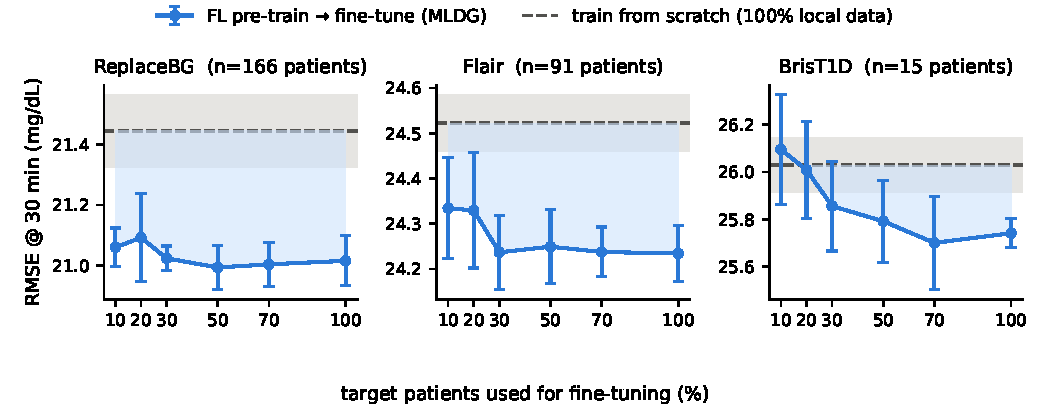
\includegraphics[width=\linewidth]{figures/data_efficiency.pdf}
\caption{\bf Data efficiency of federated pre-training.
Finetuning the MLDG-pretrained model on a fraction of each target cohort's
training patients (blue, mean $\pm$ sd over 5 seeds) against training from scratch
on $100\%$ of that cohort's patients (grey dashed, with its seed-sd band). On all
three held-out cohorts, finetuning on as little as $10\%$ of target patients
already beats from-scratch training on the full cohort; the shaded region marks
where finetuning wins. Patient counts: ReplaceBG $166$, Flair $91$, BrisT1D $15$
(so $10\%$ is $17$, $9$, and $2$ patients respectively).}
\label{fig:dataeff}
\end{figure}

\section*{Discussion}

\paragraph{Principal findings.} We federated four real adult T1D cohorts as
distinct domains and tested on three never-seen cohorts (out-of-distribution,
OOD). Federation matched single-cohort local training in-domain and
transferred more reliably out of it. Held-in, the global FedAvg and MLDG
models matched local training (average RMSE $20.09$ and $19.99$ vs.\ $20.16$
mg/dL at 30 minutes) and were within $0.1$ mg/dL of a convergence-matched
centralised model trained on the four cohorts pooled ($19.90$). OOD, on all
three held-out cohorts the federated models beat the mean single-cohort model
and avoided the collapse that the smallest-cohort model showed on each of
them. Still, most single-cohort models transferred comparably, and the mean
gain is small next to sensor error. Among the federated strategies MLDG was
numerically best in every reported comparison, but by margins within
seed-to-seed variation. These results were produced by a federation that ran
across four universities --- UCL, Manchester, Newcastle, and Oxford ---
training FedAvg, FedProx, and MLDG under the same protocol over the public
internet, with no raw data leaving any site. It is a working
multi-institution system, not a simulation.

\paragraph{Federation buys more reliable transfer, not only an accuracy gain.}
The main benefit of federation here is not in-domain accuracy --- the held-in
gap over local training is small --- but a lower risk of the collapse a
single-cohort model can suffer on data it was not trained on. A model trained
on one cohort can transfer badly: the ARISES-only model, on par with
federation on its own patients ($22.04$ vs MLDG $22.30$ mg/dL, the hardest
cohort for every method), collapsed on \emph{every} held-out cohort ($28.51
\pm 6.85$ on ReplaceBG, $32.39 \pm 5.84$ on BrisT1D, $30.99 \pm 6.23$ on
Flair). Its seed-to-seed variance was far larger than any federated model's.
The other three single-cohort models transferred within about half a mg/dL of
the federated models --- but one cannot know in advance which site's model
will fail. Every federated model avoided this failure on all three
independent held-out cohorts --- a replicated pattern, not a one-off. This is
not a guarantee (three adult cohorts do not cover the space of distribution
shift; see Limitations). But in a clinical setting, where distribution shift
is inevitable, lowering the risk of a silent, cohort-specific collapse is a
practical argument for federation independent of any in-domain accuracy
difference.

\paragraph{Generalisation versus personalisation, and how to have both.} The
results also show a tension. The personalised strategies (Ditto, APFL) and
dedicated single-cohort models were the \emph{only} approaches that beat the
federated models on the hardest and smallest in-domain cohort: on ARISES,
Ditto ($\mu{=}0.01$, $21.95$ mg/dL) and the dedicated ARISES model ($22.04$
mg/dL) edged MLDG ($22.30$). But these methods produce no single global model,
so they cannot serve the OOD cohorts at all --- the regime in which the global
models are most valuable. Specialising to a site helps that site but gives up
transfer; generalising across sites transfers but costs some per-site
accuracy. To get both, treat the global model as a foundation and adapt it
locally, rather than choosing one regime outright.

\paragraph{Finetuning a federated model for a new site.} The finetuning
experiments make the ``foundation-then-adapt'' recipe concrete, and the
pattern holds on all three held-out cohorts (Table~\ref{tab:finetune}). On
every target, finetuning a federated model beats training from scratch by
$0.3$--$0.7$ mg/dL, and improves on zero-shot transfer, most where zero-shot
was weakest. Two points follow. First, a site's own data trained in isolation
did not beat the finetuned federated model on any cohort. That is the
strongest evidence in the paper that the shared model adds something a single
site cannot recover from its own data alone. Second, which federated strategy
finetunes best depends on the cohort (FedProx on ReplaceBG, MLDG on Flair and
BrisT1D), but the three end within $\approx 0.1$ mg/dL of each other. So the
aggregation rule matters most for zero-shot transfer and washes out once
local data are available. The data-efficiency analysis
(Fig~\ref{fig:dataeff}) adds the practical point: a new site reaches, and
passes, local-only performance with roughly $10\%$ of its patients --- a
couple of dozen people, or as few as two on the smallest cohort. So the
recipe does not need a large local dataset. Beyond that point, more target
data helps little where the pool is already large (ReplaceBG, Flair) and
still helps where it is small (BrisT1D). In short: federate to get a robust
shared model, then adapt it to a new centre with a modest amount of that
centre's own data.

\paragraph{On meta-learning.} MLDG was numerically best in every reported
held-in and OOD comparison and beat FedAvg on four of five seeds. But the
margins ($\le 0.1$ mg/dL) are within seed noise, and a paired test at five
seeds does not reach significance. We therefore report a small, consistent
edge, not a demonstrated meta-learning advantage. One caveat: our MLDG splits
patients into meta-train and meta-test \emph{within} each client, so it
simulates cross-\emph{patient} shift inside a cohort, not the
cross-\emph{cohort} shift the OOD test measures. That it still comes out
consistently ahead OOD is suggestive but unexplained; a federated-DG
formulation that meta-splits \emph{across} clients would target the evaluated
shift more directly and, with more seeds to power a test, is the natural next
step. The dominant effect in our results is federation itself; the choice of
federated strategy is second-order.

\paragraph{Implications for a small group of clinics.} The case for
federating is this: a centre loses little in-domain and gains a model less
likely to fail on a population it did not train on. And since these results were themselves produced by a
four-university federation, there is evidence that the setup is practical,
not hypothetical. Because no raw record leaves any institution, federation
removes the barrier that data-protection rules such as GDPR and HIPAA place
on pooling raw data. Keeping raw data in-house is \emph{necessary but not
sufficient} for compliance: a clinical deployment would still need encryption
in transit, secure aggregation or differential privacy against inversion of
the exchanged updates, access control, and governance and impact assessment.
Our system provides none of these yet. Those are additions to a working
architecture, not obstacles to it. With those safeguards, the tooling is
light enough to run without dedicated federated-learning infrastructure. We
would expect the benefit to grow as more cohorts join and the shared model
becomes more representative, though we did not vary the number of clients and
cannot show it. Adding cohorts is also the path to something larger: a
foundation model for CGM. General time-series foundation models are already
benchmarked on glucose forecasting, where they do not yet beat a small
supervised LSTM \cite{lu2026glucofmbench} --- an argument for training on
more glucose data, not against it. Much of that data is public; much is not,
and cannot be released. Federation is one route to the part that cannot, and
it has not been tried at this scale. Our four-cohort adult T1D model is not
such a model. What we report is one ingredient --- a shared model a new site
can adapt with about a tenth of its patients --- not evidence that the larger
one would work.

\paragraph{Strengths.} Three features set this study apart from prior
federated glucose work. First, it compares local training, FedAvg, FedProx,
MLDG, and two personalised-FL families on one task under one protocol, rather
than reporting a single method in isolation. Second, it separates held-in
from OOD performance --- a distinction prior evaluations rarely make
explicit, and an informative one. The strategies are nearly indistinguishable
in-domain; OOD, the split that matters is between single-cohort training
(which can fail) and federation (which did not, here), not between federated
strategies. Third, the cohorts are split strictly by patient and normalised
with a single shared statistic, and the federation ran across four real
institutions in separate administrative domains rather than as shards of one
dataset on one host. To our knowledge these are the first federated
glucose-forecasting results from a real multi-institution run.

\paragraph{Positioning against prior results on these cohorts.} Our
per-cohort accuracy is competitive with published results on the same
datasets, under a harder protocol. The difference is the train/test split.
Almost all prior work splits each patient's series in time --- the first
portion for training, the last for testing (a \emph{by-time} split) --- so
every test window comes from a patient the model has already seen. We split
\emph{by patient}: test patients are disjoint from training patients, so every
reported number measures generalisation to people the model has never seen.
By-patient evaluation is the harder task and the one that matches deployment,
where a predictor meets new patients, but it typically yields higher error
than a by-time split on the same cohort. Table~\ref{tab:prior} collects the
closest external results. On HUPA-UCM and T1D-UOM, the strongest real-data
RMSE@30 baselines are from GlucoFM-Bench \cite{lu2026glucofmbench} (a
benchmark of time-series foundation models, univariate CGM, by-time split):
HUPA-UCM 16.71 and T1D-UOM 20.81 mg/dL. On ARISES and ABC4D they are from the
personalised meta-learning forecaster of Zhu et al.\ \cite{zhu2023fcnn} (CGM
plus carbohydrate and insulin, by-time split): 20.23 and 20.25 mg/dL. Our
by-patient figures for a global model (MLDG, numerically our best federated
strategy; HUPA-UCM 18.46, ABC4D 19.68, ARISES 22.30, T1D-UOM 19.53 mg/dL) sit
in the same 17--22 mg/dL range despite the harder split. On HUPA-UCM and
T1D-UOM they do so using CGM alone, against models that also use insulin and
carbohydrate inputs. We do not claim to beat these numbers --- a by-patient
result is not expected to --- but to match them under an evaluation that
better reflects deployment. To our knowledge no prior paper reports all four
of these cohorts, separates held-in from out-of-distribution performance, or
evaluates across-patient generalisation as we do. The one prior work that
also splits by patient (AEGIS \cite{pansheriya2026aegis}, on T1D-UOM via
leave-one-patient-out) forecasts only to 15 minutes, so it is not comparable
at our 30-minute horizon.

\begin{table}[!ht]
\centering
\captionsetup{justification=centering,singlelinecheck=on}
\caption{\bf Published RMSE@30 on our cohorts, with split protocol.}
\label{tab:prior}
\begin{tabular}{lllll}
\thickhline
study (best model) & cohort & RMSE@30 (mg/dL) & split & sd over \\
\hline
GlucoFM-Bench \cite{lu2026glucofmbench} (LSTM) & HUPA-UCM & 16.71 (4.82) & by-time & patients \\
GlucoFM-Bench \cite{lu2026glucofmbench} (LSTM) & T1D-UOM  & 20.81 (4.26) & by-time & patients \\
Zhu et al.\ \cite{zhu2023fcnn} (FCNN)          & ARISES   & 20.23 (3.38) & by-time & patients \\
Zhu et al.\ \cite{zhu2023fcnn} (FCNN)          & ABC4D    & 20.25 (2.60) & by-time & patients \\
\hline
Ours (MLDG, global)            & HUPA-UCM & 18.46 (0.28) & \emph{by-patient} & seeds \\
Ours (MLDG, global)            & ABC4D    & 19.68 & \emph{by-patient} & seeds \\
Ours (MLDG, global)            & ARISES   & 22.30 & \emph{by-patient} & seeds \\
Ours (MLDG, global)            & T1D-UOM  & 19.53 & \emph{by-patient} & seeds \\
\thickhline
\end{tabular}
\begin{center}
{\small A \emph{by-time} split tests on later windows of patients seen during
training; a \emph{by-patient} split tests on entirely unseen patients and is the
harder, deployment-relevant task. External sd is across patients; ours is across
5 seeds. Numbers are indicative, not head-to-head, because the split (and, for
Zhu et al., the input features) differ. Other papers on these cohorts report
non-comparable metrics or horizons: Tan \& McBeth \cite{tan2026uncertainty}
(MARD only), AEGIS \cite{pansheriya2026aegis} (15-min horizon, mmol/L),
Manchanda et al.\ \cite{manchanda2025lstm} (window-averaged RMSE), and Kolev
et al.\ \cite{kolev2026benchmark} (synthetic data only).}
\end{center}
\end{table}

\paragraph{Zero-shot transfer is competitive with models trained on the target
cohort.} The comparison above concerns the cohorts we trained on. The sharper
test is a cohort we have \emph{never seen}, against models developed on it.
ReplaceBG allows this comparison: two studies report 30-minute RMSE on it
under the same protocol we use --- a by-patient hold-out, on a 5-minute grid,
as a point error at the 30-minute horizon. The only difference is that they
trained on ReplaceBG and we did not (Table~\ref{tab:oodprior}). Our federated
MLDG model reaches $21.34$ mg/dL on ReplaceBG having never seen any of its
patients. That places it inside the field of models developed on the cohort.
It beats an in-distribution Bi-LSTM ($21.7$), GRU ($22.1$), ARIMA ($28.1$)
and SVR ($37.4$), and is level with N-BEATS ($21.2$), TCN ($21.3$) and
Crossformer ($21.1$). It trails only GluLLM ($20.6$, which also uses insulin
and electronic-health-record features we do not) and GPFormer ($19.2$), which
was trained centrally on ReplaceBG itself. Three caveats apply. First, the
$2.1$ mg/dL gap to GPFormer mixes two differences: GPFormer both trained on
the target cohort \emph{and} uses sparse attention where ours uses full
attention, so the gap is not a clean measure of the cost of federation alone.
Second, the test sets are not identical: the published studies evaluate on a
46-subject hold-out from a model \emph{trained on the rest of ReplaceBG}. We
evaluate on a 21-patient test split from a model that never saw \emph{any}
ReplaceBG patient. Both test on unseen individuals; only ours also faces an
unseen cohort --- a different, and arguably harder, setting. Third, reported
ReplaceBG results vary widely with protocol: one study reports $9.3$ mg/dL
\cite{jaloli2023cnnlstm}, but on a 15-minute grid and with a rolling split
that re-admits test patients to training. That is not comparable to any of
the numbers here. With those caveats, the point stands: a model that never
saw ReplaceBG, and never pooled raw data from anywhere, lands inside the
field of models developed on it.

This parity is specific to the 30-minute horizon; it does not survive at 60
minutes. There, our zero-shot MLDG reaches $36.49$ mg/dL on ReplaceBG
(Table~\ref{tab:h60}) against $32.3$ for GPFormer, $34.1$ for N-BEATS and
$34.7$ for Bi-LSTM \cite{zhu2024gpformer} --- behind \emph{every}
in-distribution baseline rather than among them. The likely reason: at short
horizons a forecaster relies on recent CGM dynamics, which transfer across
cohorts, so a model trained elsewhere loses little. At longer horizons
prediction depends more on cohort-specific behaviour --- meal and insulin
routines, treatment regimen, sensor characteristics --- which a model that
never saw the cohort does not know. Zero-shot federation buys parity where
shared physiology dominates the task, and pays a growing price where
cohort-specific habit dominates. For the 30-minute alerting use case that
motivates this work, the first regime is the relevant one; for longer-range
planning, local data are worth more.

\begin{table}[!ht]
\centering
\captionsetup{justification=centering,singlelinecheck=on}
\caption{\bf Our zero-shot result on ReplaceBG against models trained on ReplaceBG.}
\label{tab:oodprior}
\begin{tabular}{llcc}
\thickhline
model & inputs & trained on ReplaceBG & RMSE@30 \\
\hline
GPFormer \cite{zhu2024gpformer}    & CGM                & yes & $19.2$ \\
GluLLM \cite{zhu2026glullm}        & CGM + insulin + EHR & yes & $20.6$ \\
Crossformer \cite{zhu2026glullm}   & CGM + insulin + EHR & yes & $21.1$ \\
N-BEATS \cite{zhu2024gpformer}     & CGM                & yes & $21.2$ \\
TCN \cite{zhu2026glullm}           & CGM + insulin + EHR & yes & $21.3$ \\
\textbf{Ours --- MLDG (federated)} & \textbf{CGM}       & \textbf{no} & $\mathbf{21.34}$ \\
\textbf{Ours --- FedAvg}           & \textbf{CGM}       & \textbf{no} & $\mathbf{21.43}$ \\
\textbf{Ours --- FedProx}          & \textbf{CGM}       & \textbf{no} & $\mathbf{21.57}$ \\
Bi-LSTM \cite{zhu2024gpformer}     & CGM                & yes & $21.7$ \\
GRU \cite{zhu2026glullm}           & CGM + insulin + EHR & yes & $22.1$ \\
ARIMA \cite{zhu2024gpformer}       & CGM                & yes & $28.1$ \\
SVR \cite{zhu2024gpformer}         & CGM                & yes & $37.4$ \\
\thickhline
\end{tabular}
\begin{center}
{\small RMSE (mg/dL) at the 30-minute horizon on ReplaceBG. All rows use a
by-patient hold-out on a 5-minute grid and report a \emph{point} error at 30
minutes (not a window average). Every published row was \emph{trained on
ReplaceBG}; our three rows were trained on four entirely different cohorts and
never saw ReplaceBG, so they are zero-shot. Published values are read from
\cite{zhu2024gpformer,zhu2026glullm}; those two sources evaluate on the same
46-subject hold-out of ReplaceBG, whereas our models are evaluated on a 21-patient
test split of ReplaceBG that, like all ReplaceBG patients, was never seen in
training. Note that GPFormer additionally uses sparse attention while our
forecaster uses full attention, so the GPFormer--ours gap reflects architecture as
well as training regime.}
\end{center}
\end{table}

\paragraph{BrisT1D and Flair are, to our knowledge, previously unbenchmarked.}
We report $26.31$ and $25.05$ mg/dL on these two cohorts but make no
comparative claim: we could find no published 30-minute-horizon RMSE in mg/dL
on either. The BrisT1D Kaggle competition \cite{kaggle2024brist1d} targets a
\emph{60-minute} horizon in mmol/L and so is not comparable, the published
models that use BrisT1D report errors on a normalised scale, and for Flair we
found no glucose-forecasting benchmark at all. We therefore offer these two
numbers as zero-shot reference points for future work rather than as wins.
One property of Flair matters here: it is a hybrid closed-loop (automated
insulin delivery) cohort \cite{bergenstal2021flair}, and automated delivery
suppresses glycaemic variability, which tends to make forecasting easier. Its
lower error relative to BrisT1D partly reflects the cohort rather than the
model. The value of
these two cohorts is not that we beat anyone on them --- it is that the
federated models behave consistently on three independent unseen populations
while a single-cohort model collapses on all three.

\paragraph{Limitations.} Several constraints bound these conclusions.
\emph{(i) Evaluation metric.} We report a single aggregate error (RMSE at 30
min). This lags the studies we compare against, which report clinical error grids
(Clarke/Parkes), MARD, or hypo-/hyperglycaemia detection; aggregate RMSE is
dominated by the euglycaemic range and can be near-blind to the
safety-critical hypoglycaemic tail. Our model also emits a point forecast with
no calibrated predictive uncertainty. Whether federation's small advantage
survives on clinically stratified and event-detection metrics is untested; a
full error-grid analysis is the most important gap for a clinical reading of
this work.
\emph{(ii) OOD breadth and composition.} Our transfer claim rests on three
held-out cohorts (ReplaceBG, BrisT1D, Flair). None covers paediatric or type-2
populations, and the three are not equivalent tests. Flair is a hybrid
closed-loop (automated insulin delivery) cohort of adolescents and young
adults, whose suppressed glycaemic variability makes forecasting easier;
BrisT1D is a small (24-participant) open-loop young-adult cohort.
Absolute errors are therefore not comparable \emph{across} the three cohorts;
only the within-cohort ranking of strategies is. A leave-one-cohort-out design
would probe transfer further. \emph{(iii) Statistical power.} Margins among federated strategies
($\le 0.1$ mg/dL) are within seed standard deviation and a paired test at five
seeds does not reach significance, so we do not claim a ranking; MLDG's
consistency (best in every comparison, 4/5 seeds) is suggestive but underpowered.
Seed sd also reflects one fixed patient split and understates patient-sampling
uncertainty. \emph{(iv) Baselines.} We include no persistence or simple
learned baseline in the main table, so we cannot fully attribute accuracy to
the transformer versus the training scheme; FedProx used a single untuned
$\mu$. (APFL, by contrast, is not under-tuned: its mixing weight is learned,
and we report where it converges.) \emph{(v) Horizon.} We report the 30- and
60-minute horizons; the model does not forecast beyond 60 minutes, so the 90-
and 120-minute horizons some comparators report are out of scope. Our parity
with in-distribution models on ReplaceBG holds at 30 minutes but not at 60.
\emph{(vi) Privacy and jurisdiction.} Raw data never moves, but the system
provides no formal guarantee: it uses plain HTTP without encryption, secure
aggregation, or differential privacy, and the exchanged updates could in
principle be attacked. All four sites are within one country, so the legal and
governance complexity of a cross-border federation remains untested.
\emph{(vii) Population.} All seven cohorts are adult T1D, leaving paediatric
and type-2 transfer untested, and we scope the benchmark to meta-learning and
personalisation, leaving representation-alignment methods to future work.
\emph{(viii) Mechanism.} The centralised reference shows that federation
recovers the accuracy of pooling, and the single-cohort collapse shows that
data diversity is what buys reliable transfer. The mechanism should be read
as ``more diverse training data, obtained under a privacy constraint'', not
anything specific to federated averaging itself.

\paragraph{Future work.} The next steps follow from these limitations. First:
add clinical metrics --- a full Clarke/Parkes error grid, MARD, and
event-level hypo-/hyperglycaemia detection with predictive uncertainty --- to
test whether federation's advantage holds where safety matters. Add
persistence and simple learned baselines. Add more seeds to power the
strategy comparison. And run a leave-one-cohort-out evaluation to extend
transfer testing beyond the three held-out cohorts. Beyond that: add
event-aware inputs such as insulin and carbohydrate information. Add secure
aggregation and differential privacy so that keeping raw data in place
carries a formal guarantee. And extend the four-institution federation across
national borders, reporting communication, latency, straggler, and failure
behaviour under cross-jurisdiction governance. Finally, our finetuning is a
two-stage pipeline (federate, then adapt); training the global model and its
per-site specialisations \emph{jointly}, and continual federation as
populations and devices drift, are natural extensions this framework is set
up to support.


% ===========================================================================
% Compile references.bib with the plos2025.bst style (ships with PLOS template).
\bibliography{references}

\end{document}
